{
% \usebackgroundtemplate{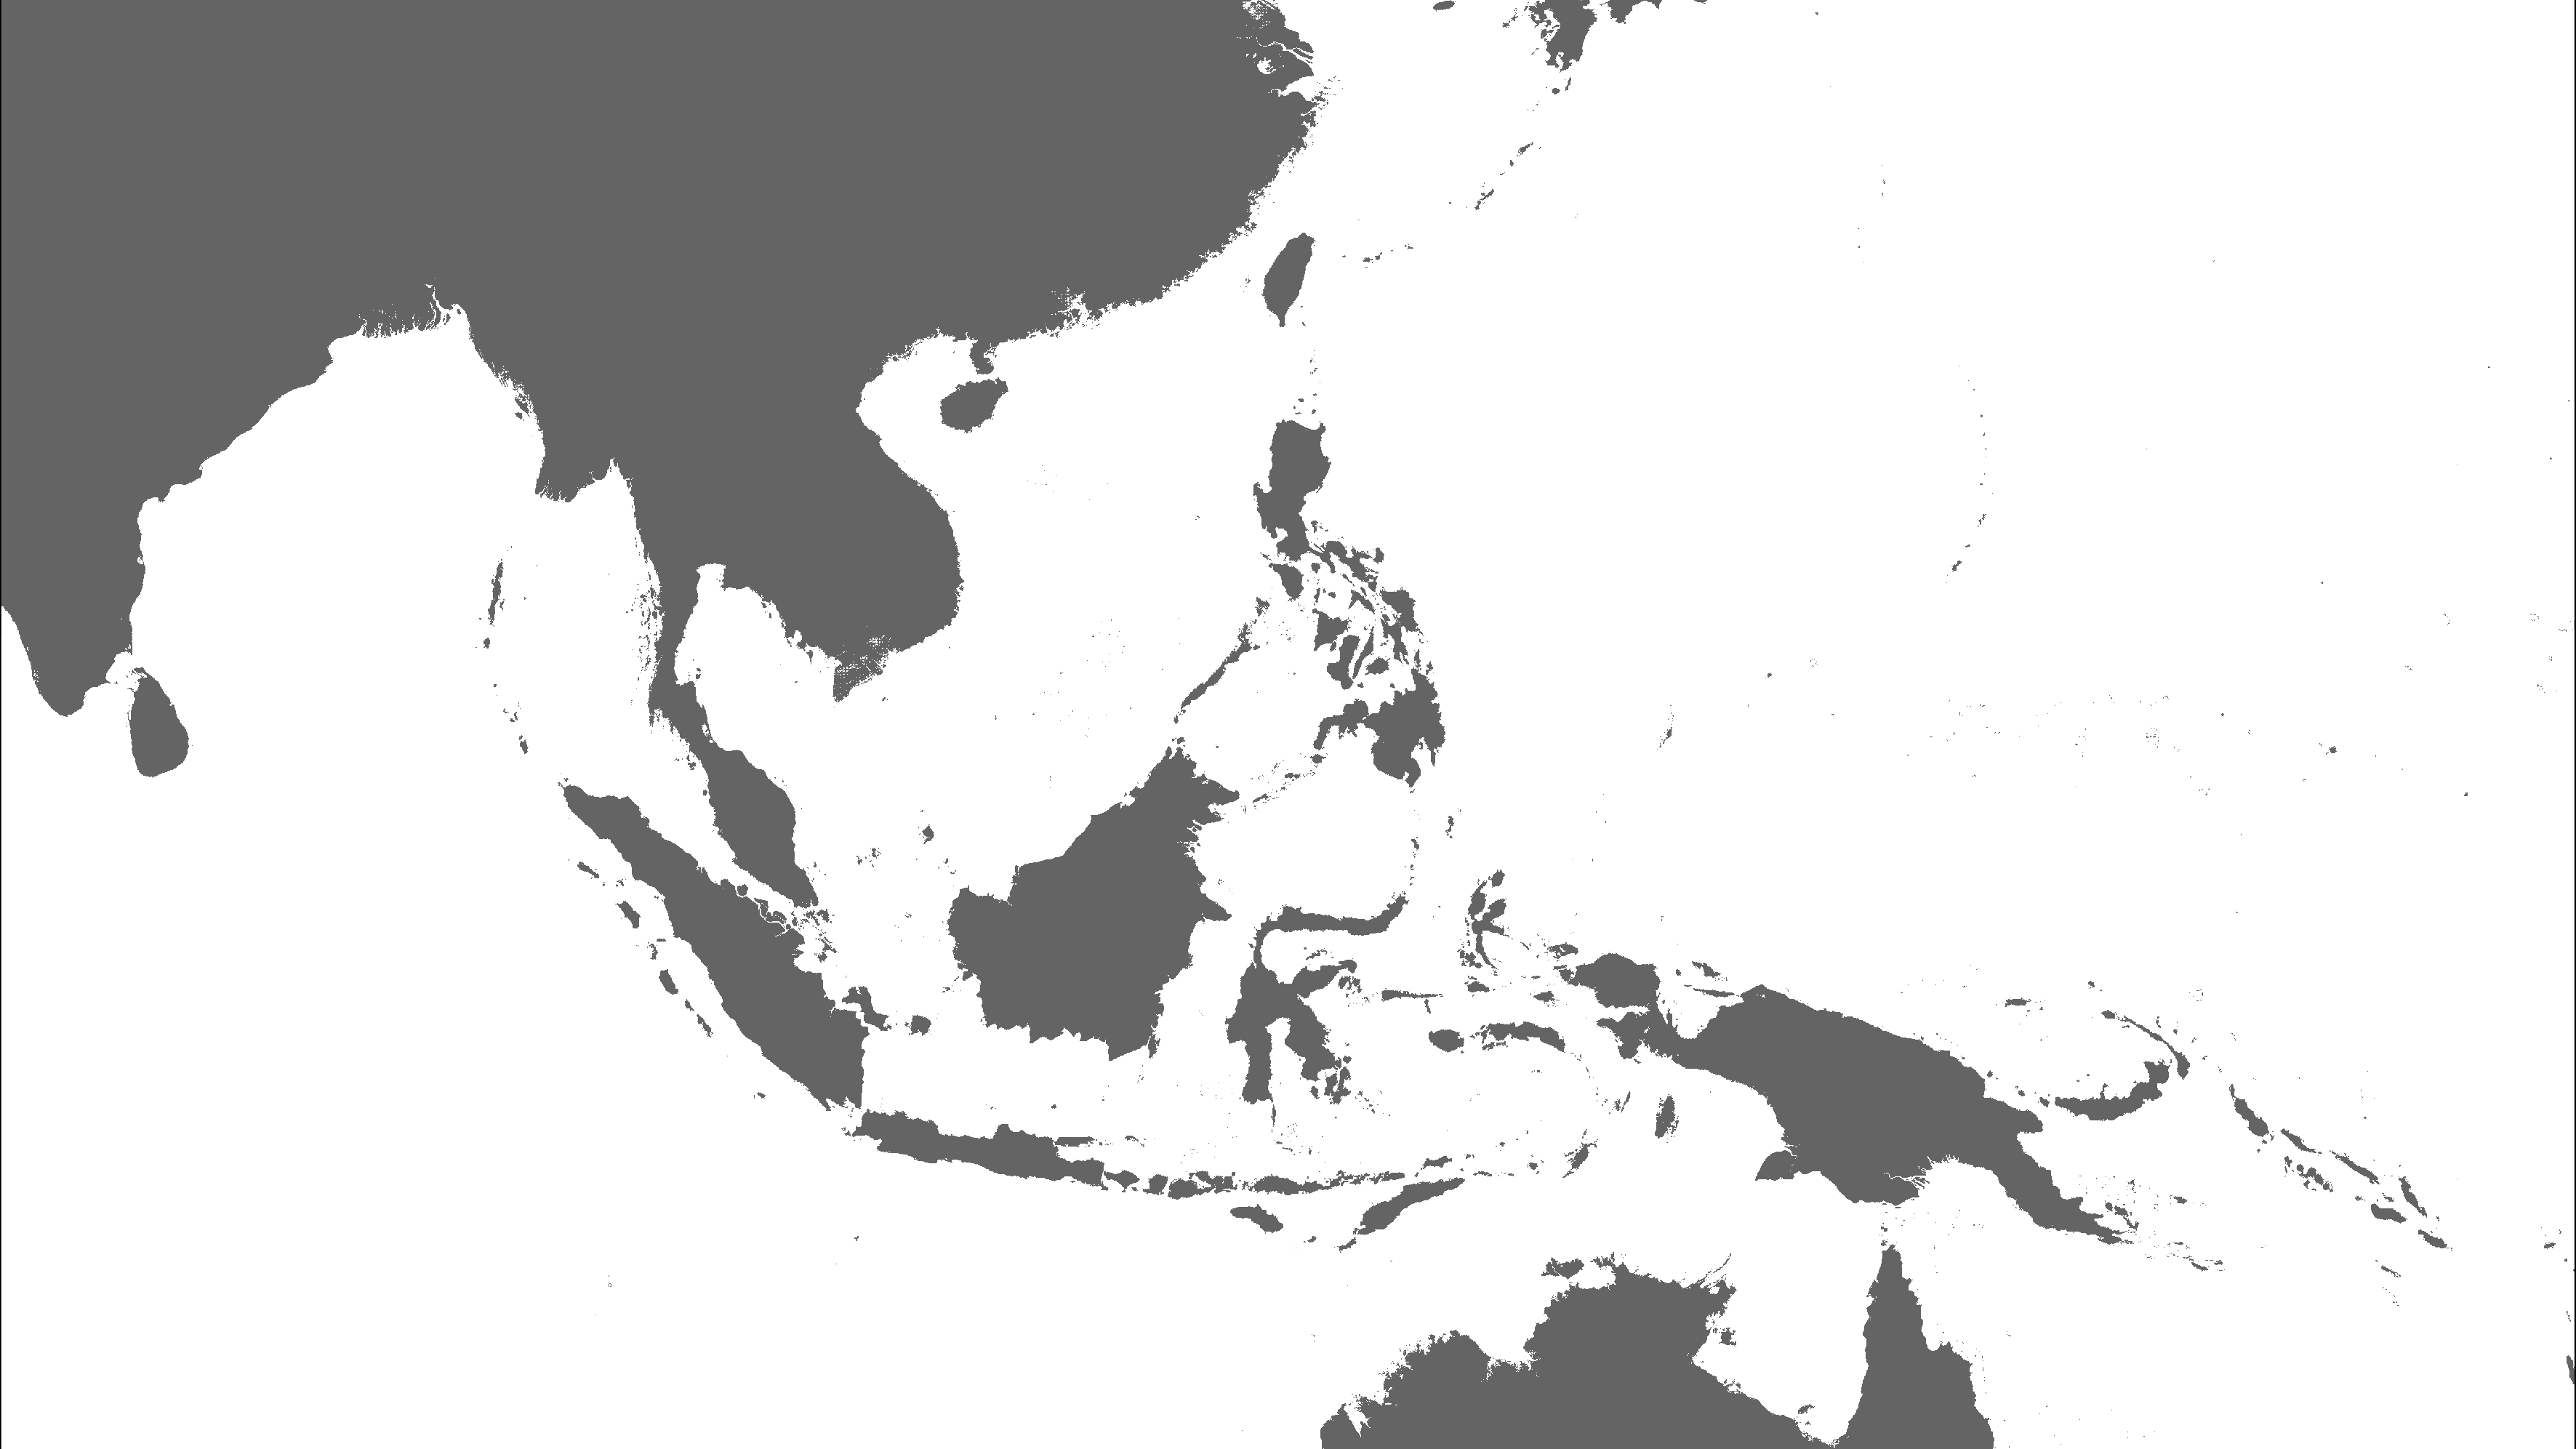
\includegraphics[width=\paperwidth]{../images/se-asia-present-widescreen.png}}
\usebackgroundtemplate{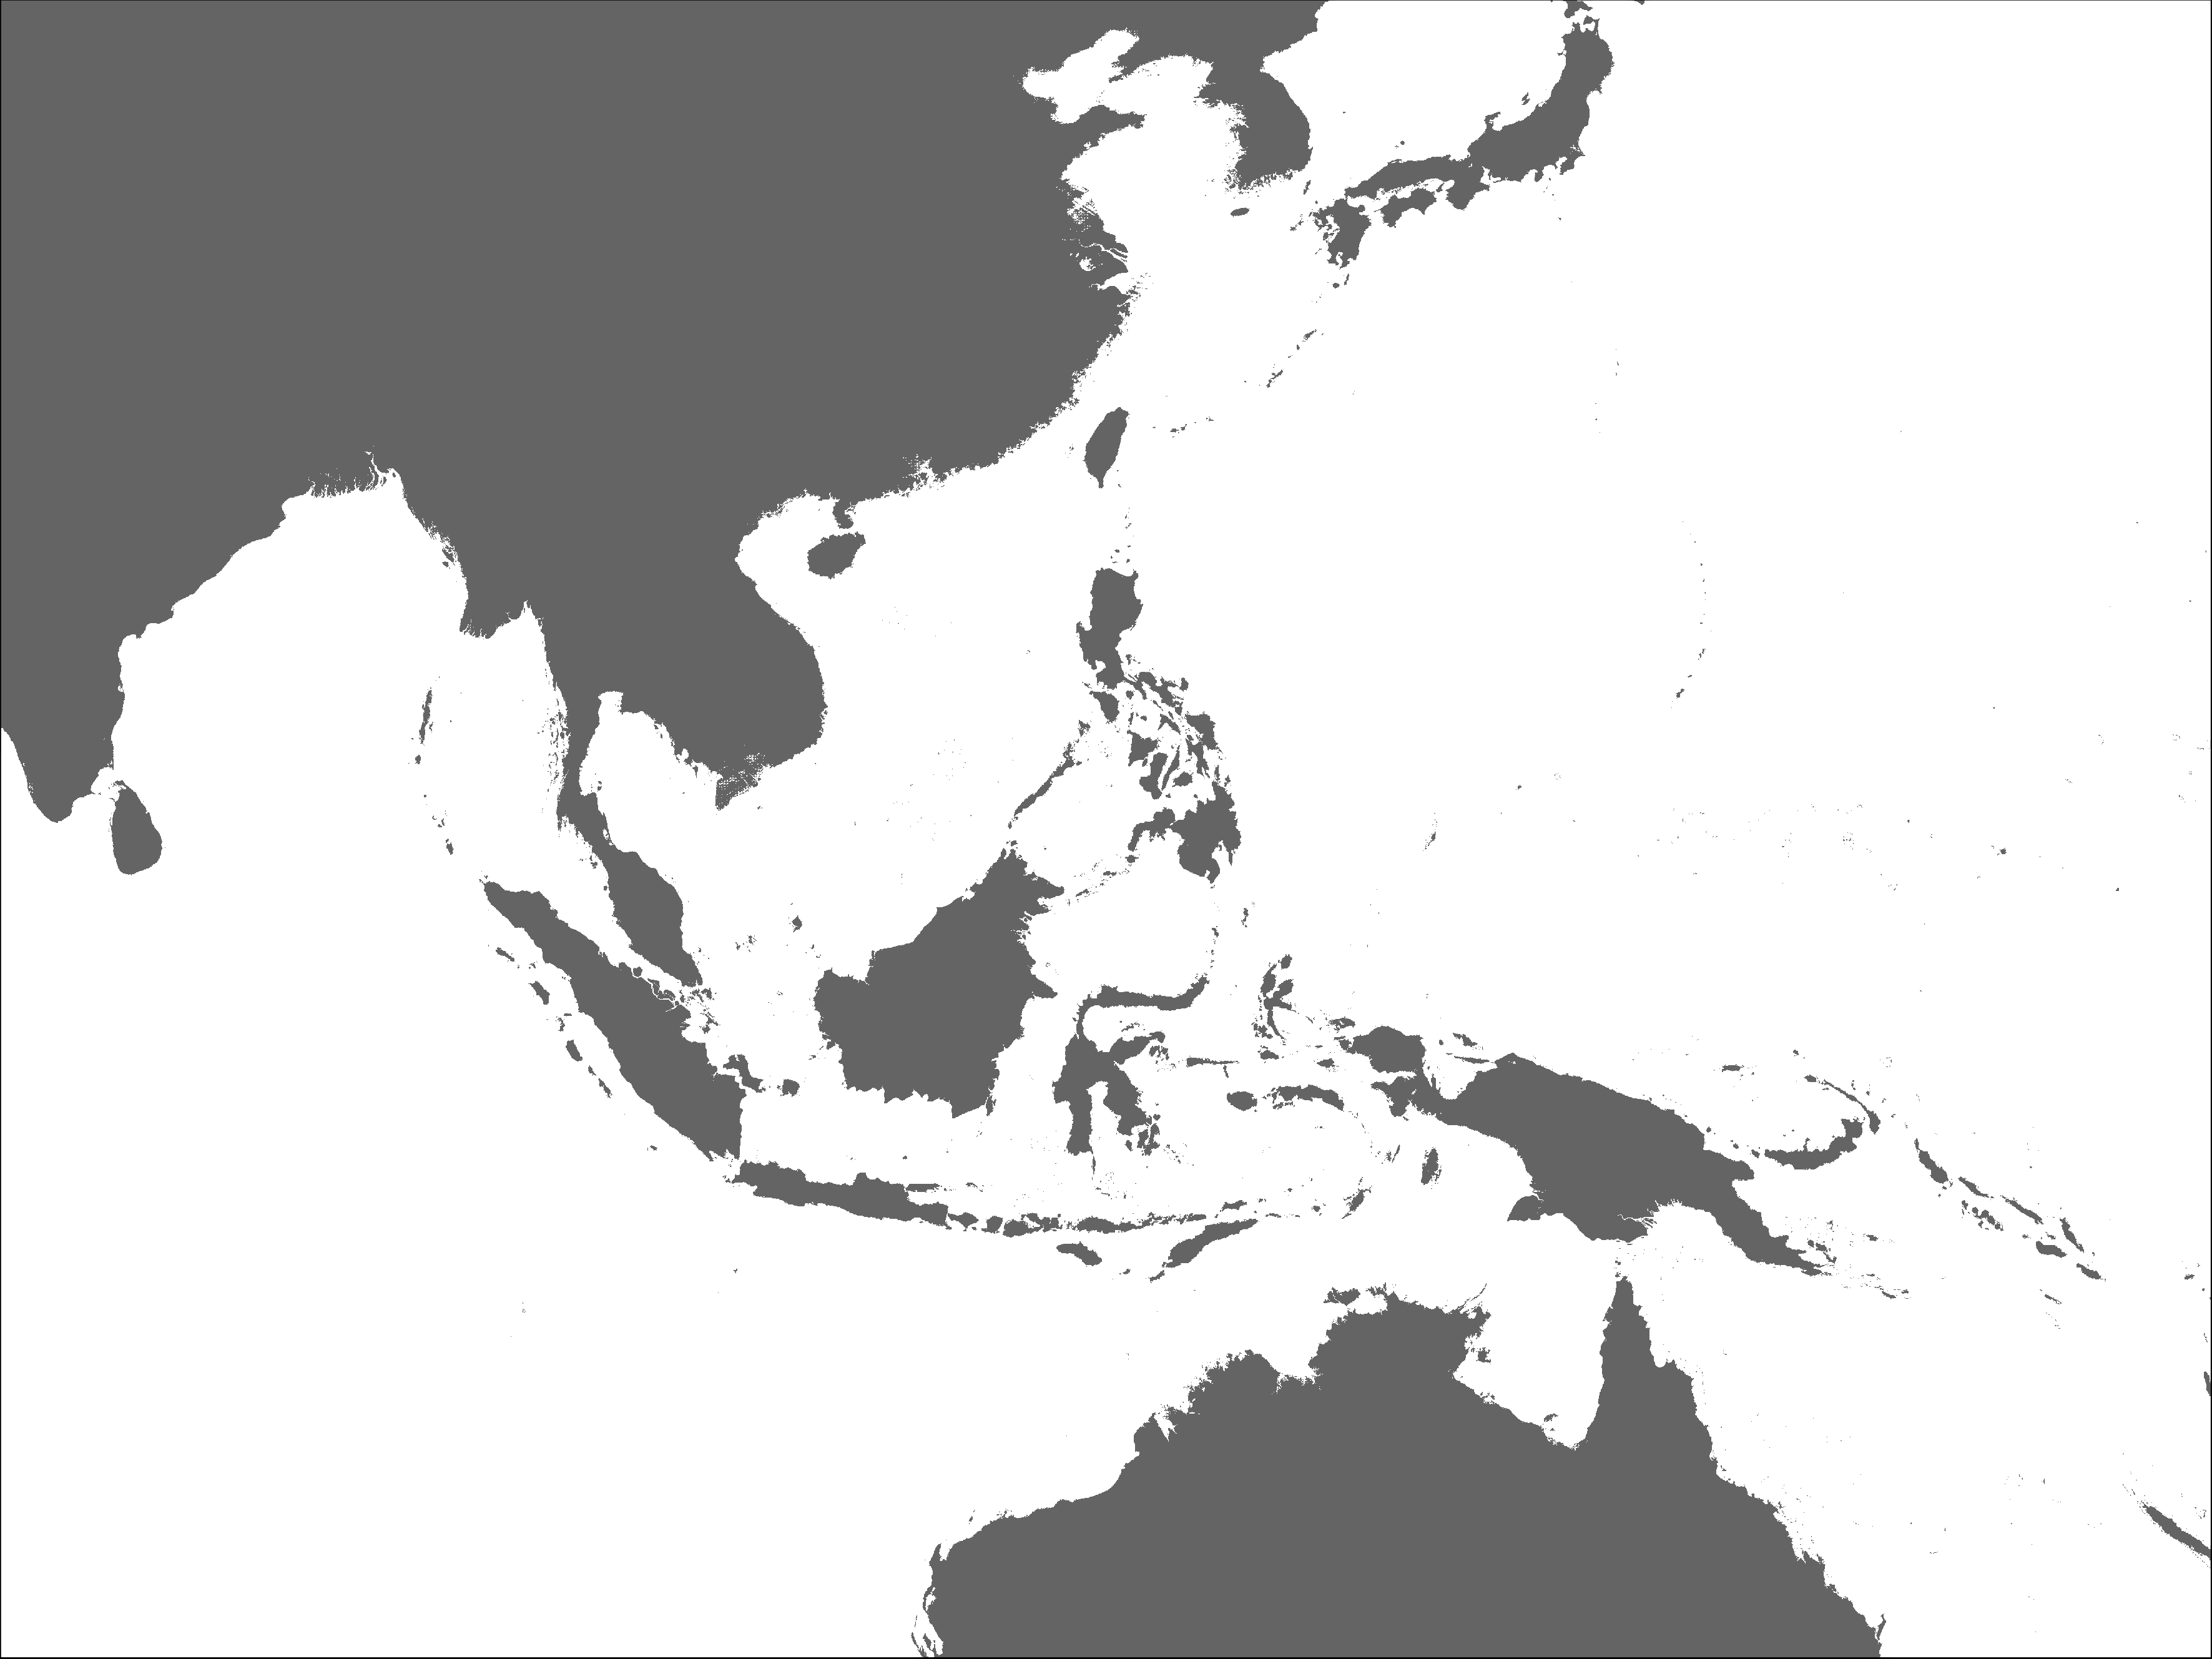
\includegraphics[width=\paperwidth]{../images/se-asia-present.png}}
\begin{frame}
    % \frametitle{Empirical applications}    
\end{frame}
}
{
% \usebackgroundtemplate{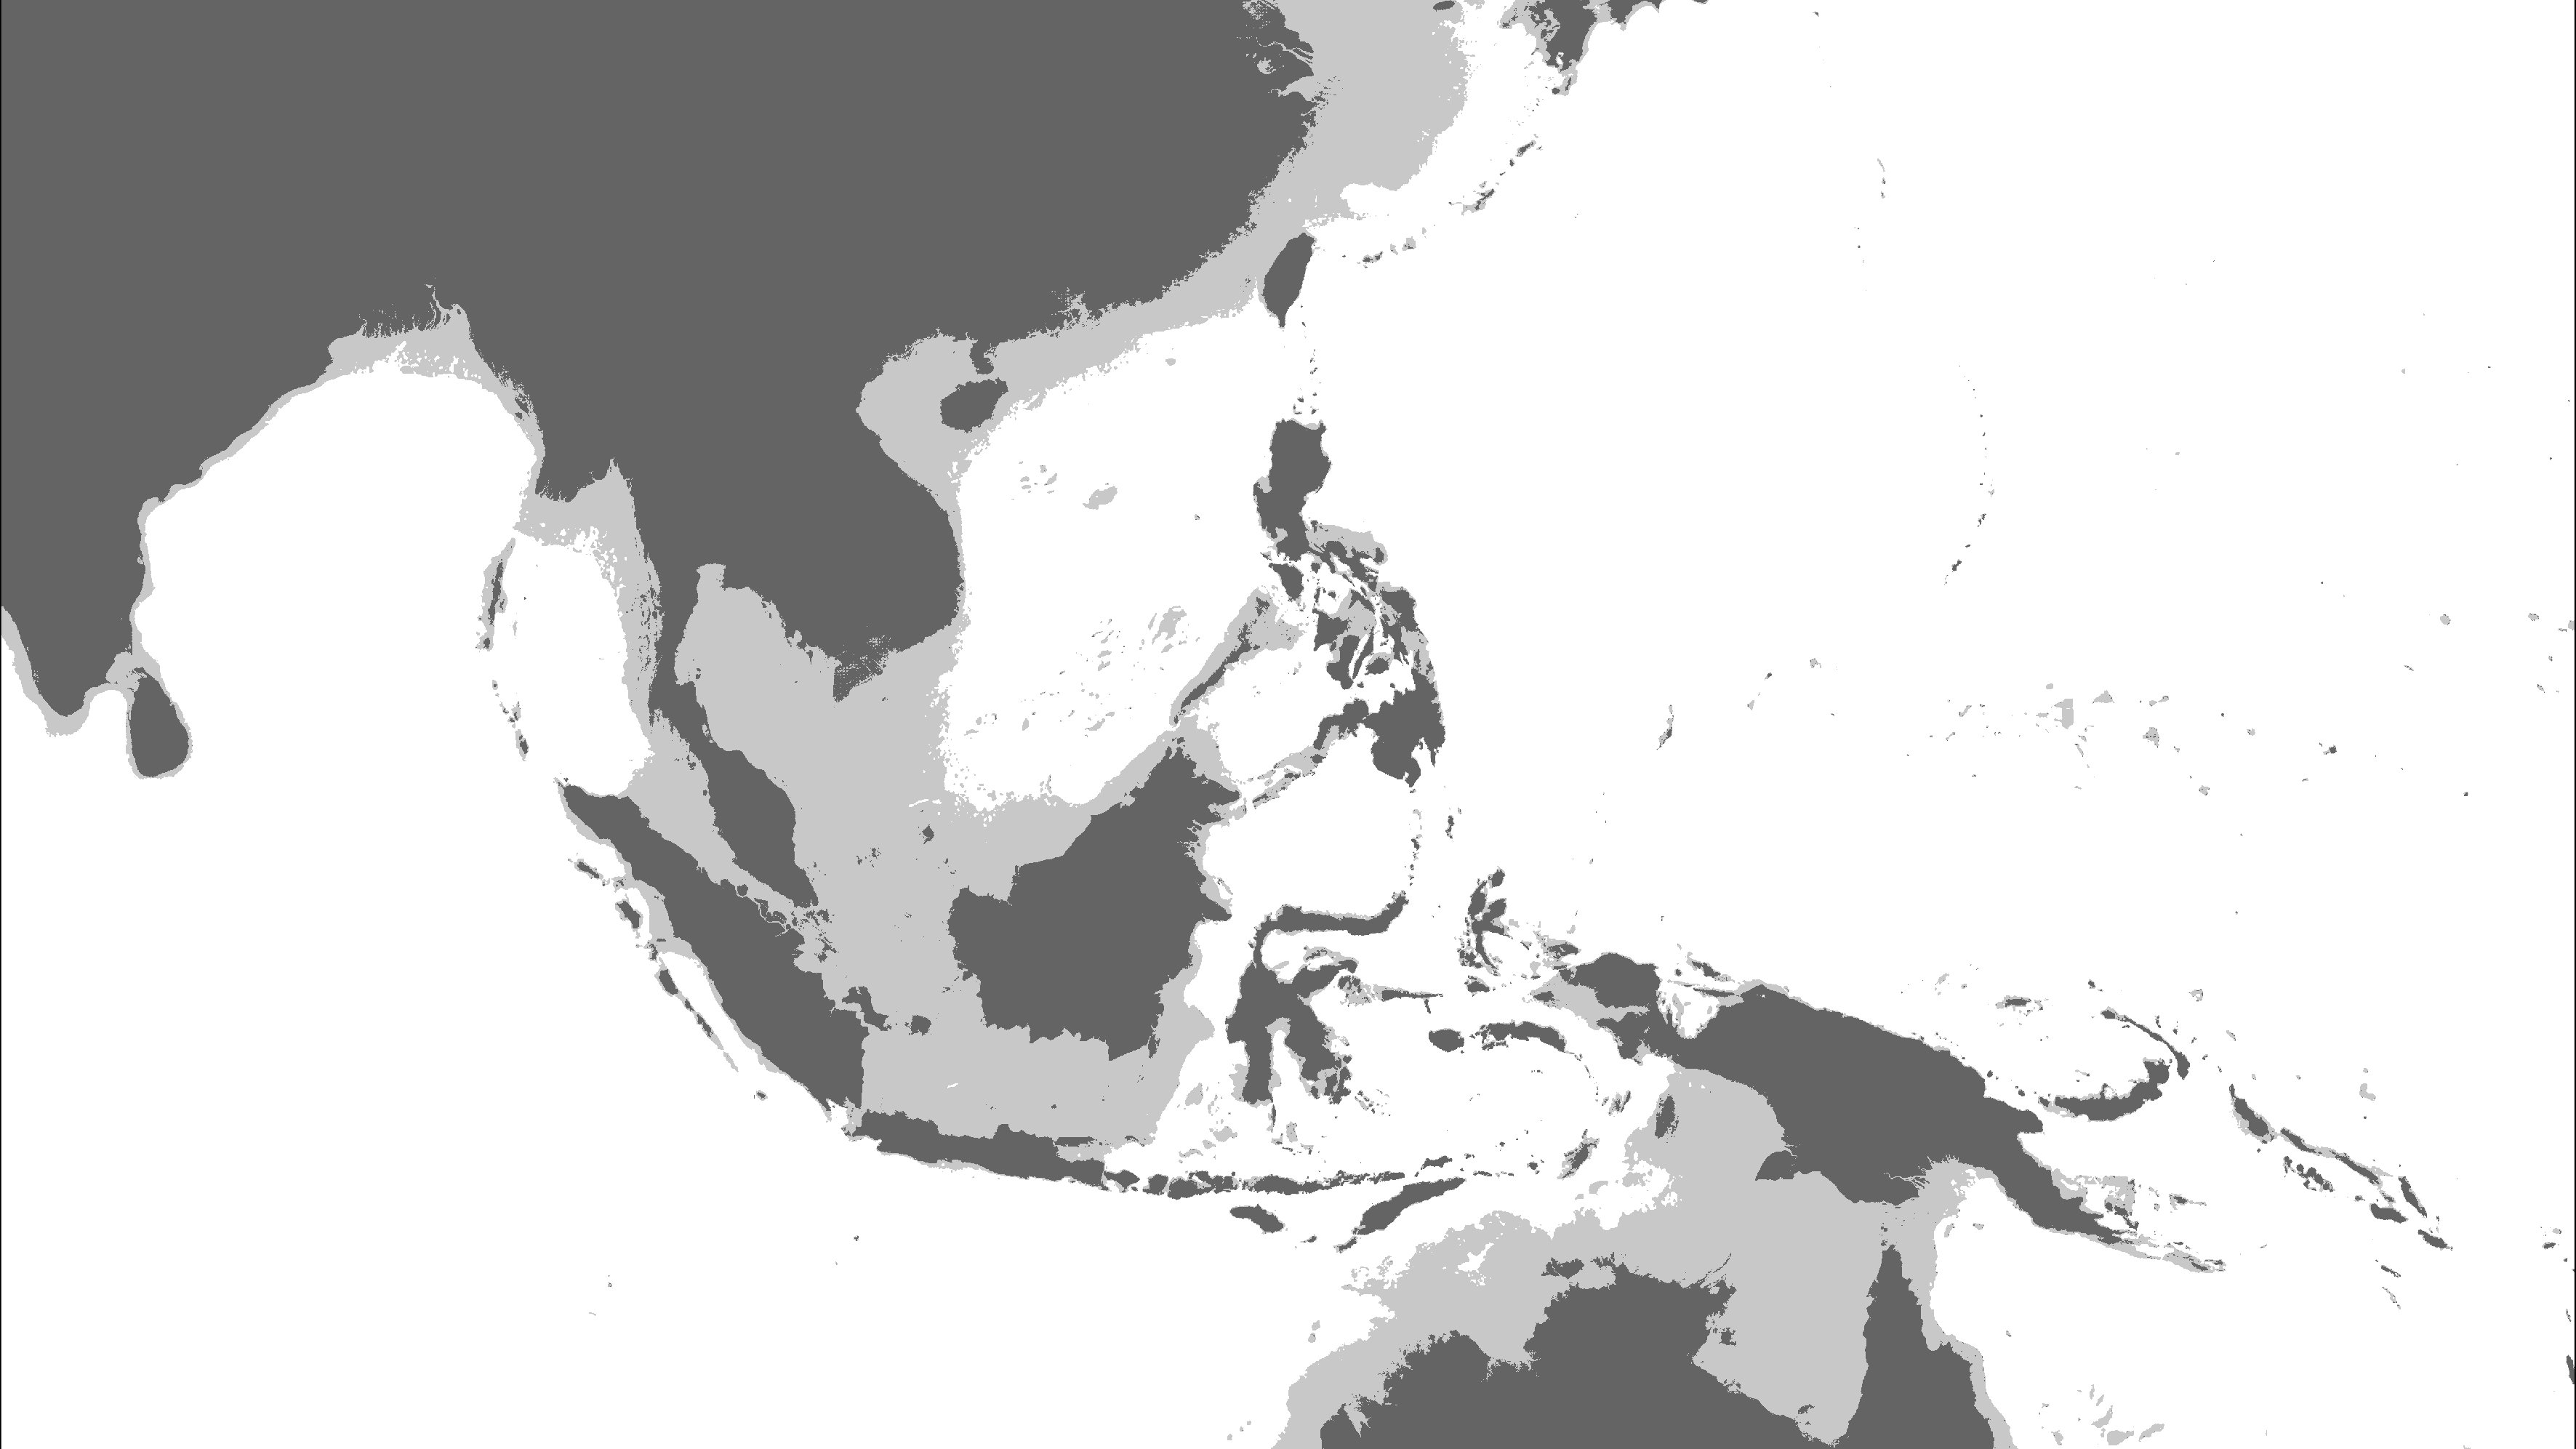
\includegraphics[width=\paperwidth]{../images/se-asia-120-widescreen.png}}
\usebackgroundtemplate{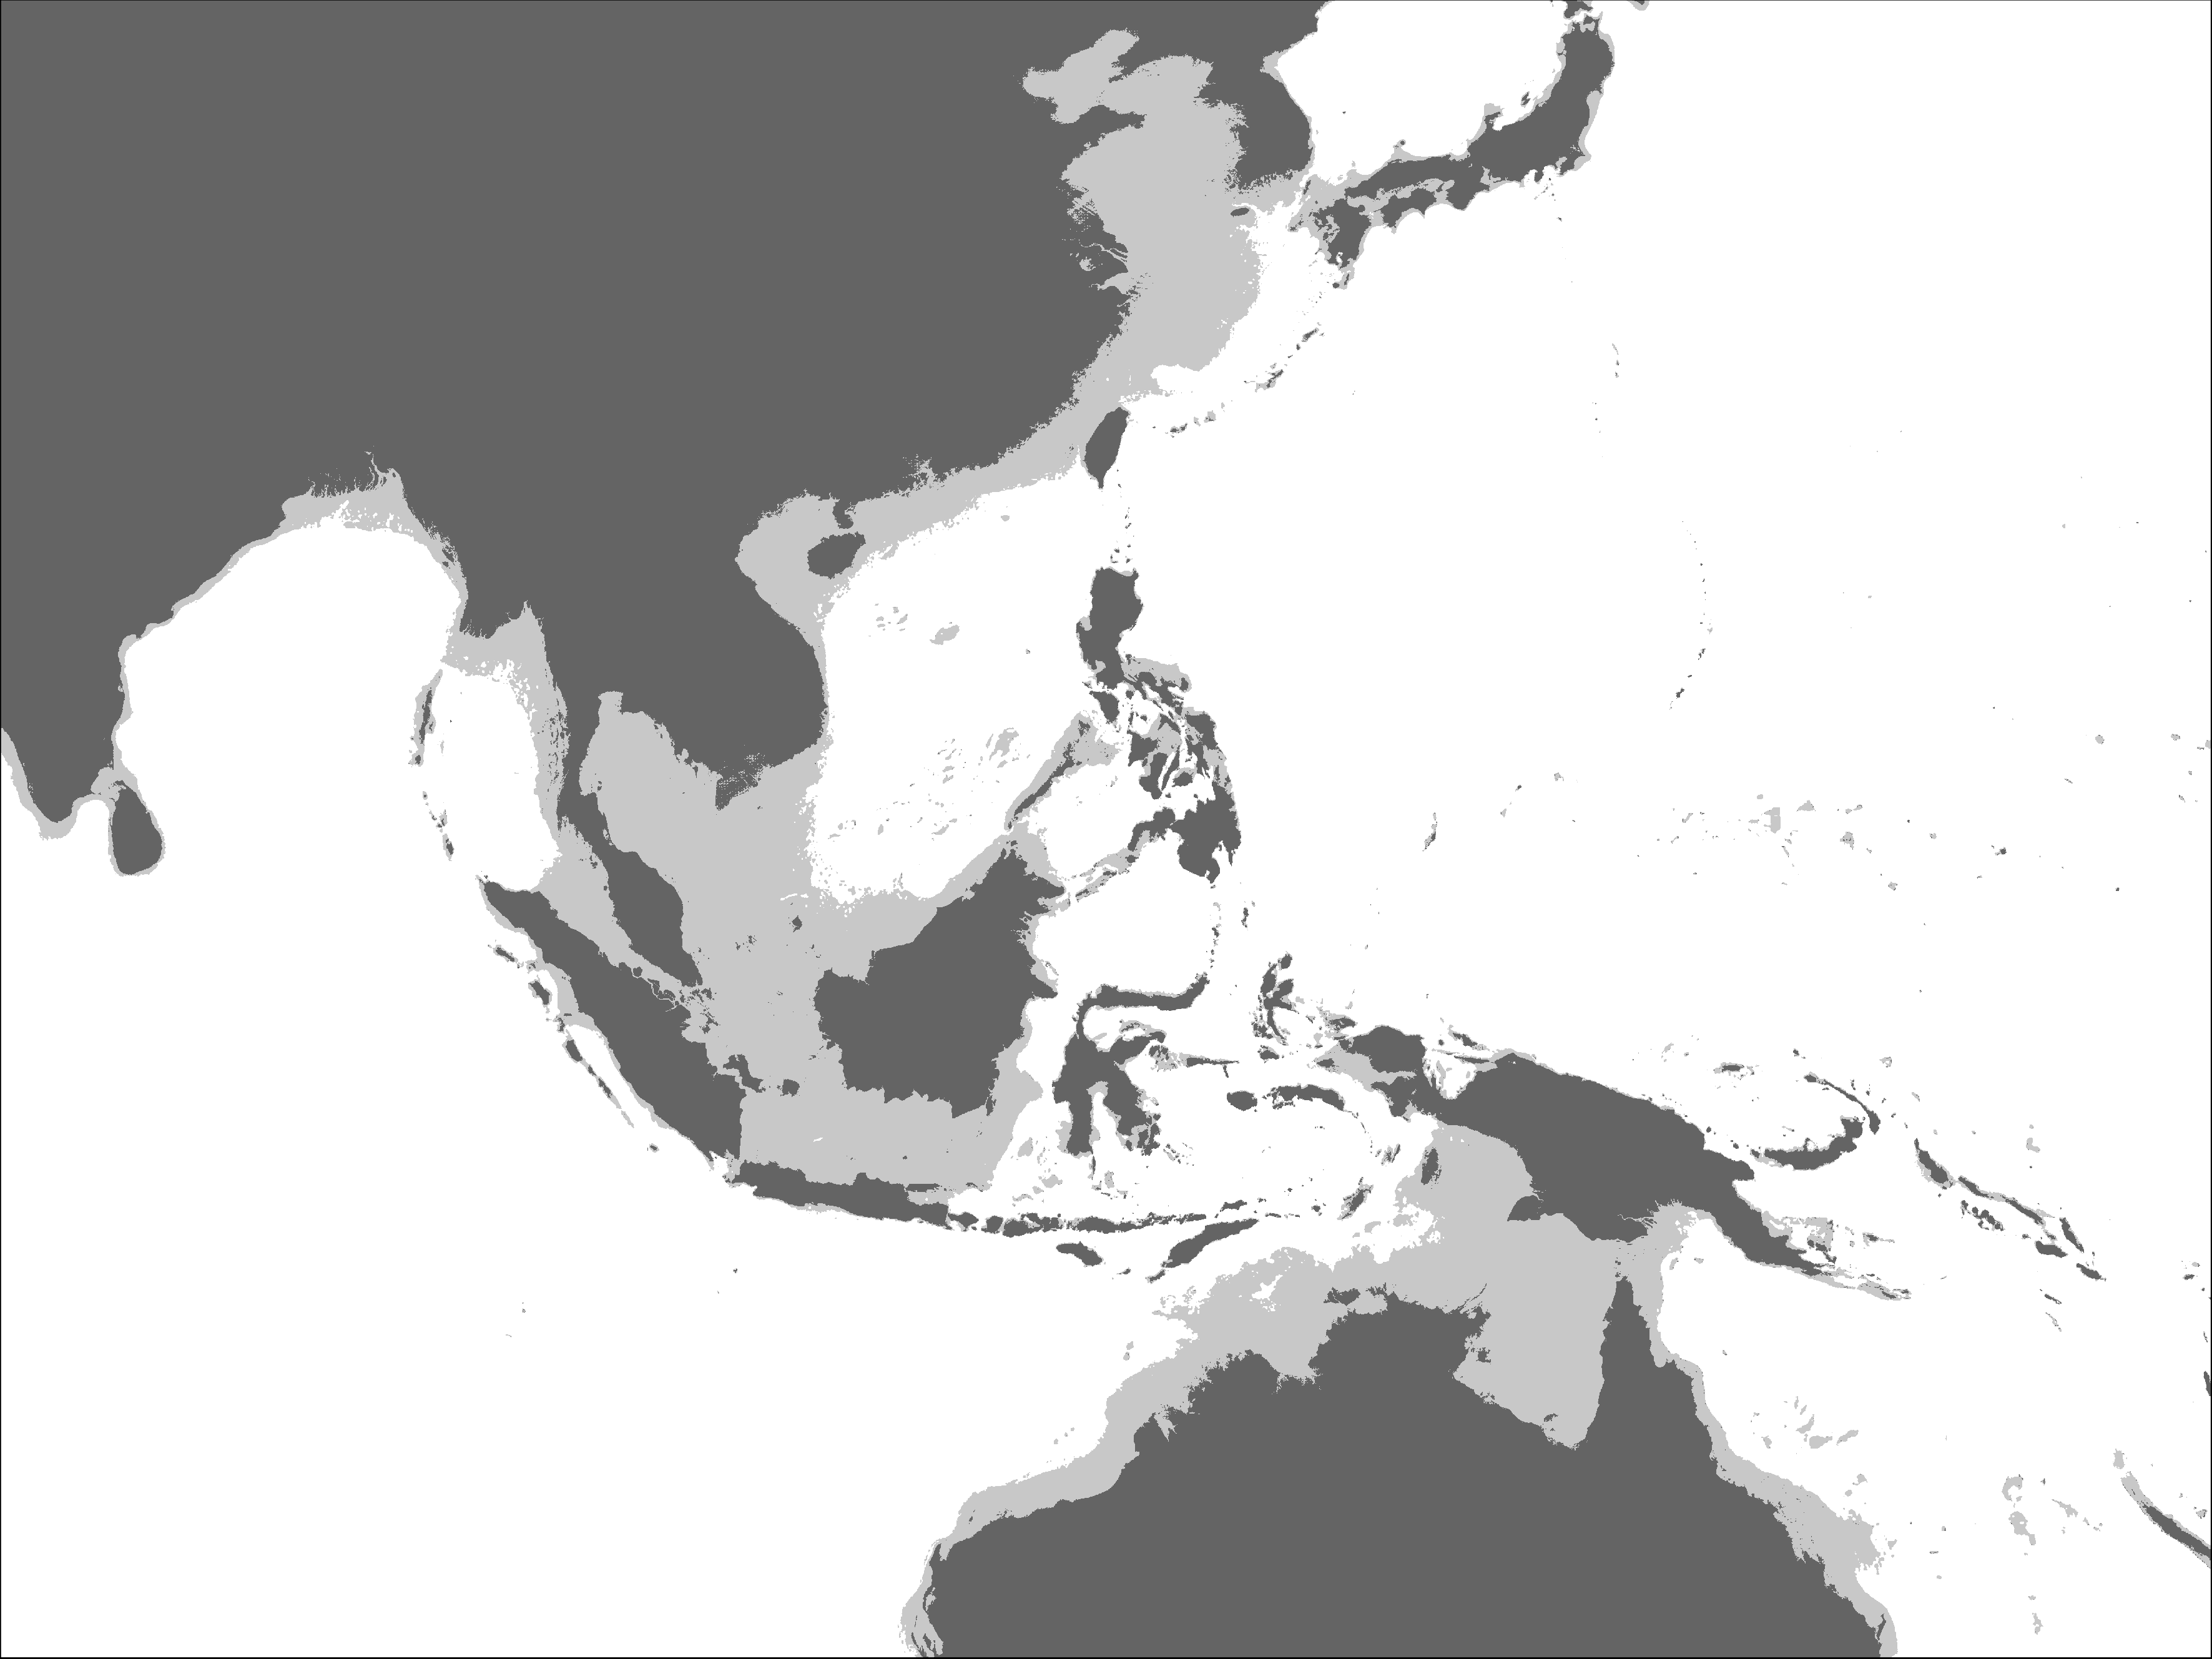
\includegraphics[width=\paperwidth]{../images/se-asia-120.png}}
\begin{frame}
    % \frametitle{Empirical applications}    
    \begin{columns}
        \column{0.56\textwidth}

        \vspace{6.5cm}

        \begin{uncoverenv}<3->
        \colorbox{white}{
            \begin{minipage}[t]{0.6\textwidth}
                \raggedright
                See a
                \href{https://youtu.be/mLNLRdbu5W8}{sea-level animation of SE Asia here}
            \end{minipage}
        }
        \end{uncoverenv}

        \ \\

        \column{0.4\textwidth}

        \vspace{-2cm}

        \begin{uncoverenv}<2->
        \colorbox{white}{
            \begin{minipage}[t]{1.0\textwidth}
                \raggedright
                \textbf{Did repeated fragmentation of islands during
                    inter-glacial rises in sea level promote diversification?}
            \end{minipage}
        }
        \end{uncoverenv}
    \end{columns}
\end{frame}
}
